\documentclass[11pt]{article}
\usepackage[margin=0.7in]{geometry}
\usepackage{amsmath}
\usepackage{graphicx}

\begin{document}

\title{Accounting for non-CO$_2$ forcing in outstanding carbon budgets}
\author{Stuart Jenkins}
\date{06/02/19}
\maketitle

\section{Introduction}

\section{Defining the carbon budget for multi-gas scenarios}

Remaining warming is, for an ambitious mitigation scenario in which temperatures peak well before 2100 and non-CO$_2$ forcing increases or declines smoothly between now and the time of peak warming, well approximated by

\begin{equation}
    \Delta T = (\text{TCRE} \times G) + \frac{\text{TCR} \times (F_1 - F_0)}{F_{2\text{x}}} + \frac{[(\text{ECS}-\text{TCR})\times\Delta t \times F_0]}{d_2 \times F_{2\text{x}}}
\end{equation}
where $G$ is the cumulative remaining carbon budget to peak warming, $F_0$
is the mean global effective non-CO$_2$ foricng over the past 10-20 years, $F_1$ is the mean global effective non-CO$_2$ forcing over the 10-20 years prior to peak warming, $F_{2\text{x}}$ is the forcing due to doubled CO$_2$, $d_2$ is the long thermal response-time of the climate system and $\Delta t$ is the time to peak warming. 

Using the relationship $\text{TCR} = F_{2\text{x}} \times \text{TCRE} \times \text{H } / \text{ AGWP}_\text{H}$, as noted in Allen \textit{et al.}, 2018 ('A solution to the misrepresentation of CO$_2$ equivalent emissions of short-lived climate pollutants under ambitious mitigation') we find

\begin{equation}
    \Delta T = \text{TCRE} \times \Big[G + \frac{\text{H}\times(F_1 - F_0 + \epsilon\Delta t F_0)}{\text{ AGWP}_\text{H}}\Big]
\end{equation}

where AGWP$_\text{H}$ is the AGWP of CO$_2$ over a time-horizon of H, and $\epsilon = \frac{(\text{ECS}-\text{TCR})}{\text{TCR} \times d_2}$. Therefore, $\epsilon$ represents the fractional rate of forcing decline required to maintain stable temperatures (around 0.3\% per year). Flipping the above equation we can find the remaining carbon budget to a further $\Delta T$ degrees warming:

\begin{equation} \label{cum_carbon_eq}
    G = \frac{\Delta T}{\text{TCRE}} - \frac{\text{H} \times (F_1 - F_0 + \epsilon\Delta t F_0)}{\text{AGWP}_{\text{H}}}.
\end{equation}

This makes it nice and clear how non-CO$_2$ forcing translates into CO$_2$-forcing-equivalent emissions (and hence how individual components could also be expressed in this way). All of the quantities in these equations (ECS, TCR, d$_2$, AGWP$_\text{H}$, TCRE) are going to be assessed in AR6, and it will therefore be straightforward for anyone to assess whether they are consistent with estimated remaining carbon budgets.

\section{The remaining budget for ambitious mitigation scenarios}

As a first assessment of the accuracy of equation \ref{cum_carbon_eq}, we check the estimated remaining carbon budgets for the IIASA database of $1.5^{\circ}$C-compatible scenarios (no-, low- and high-overshoot scenarios). First running the scenarios through FaIR we find the temperature response to each scenario, and therefore remaining warming to peak warming, $\Delta T$, and the time to peak warming, $\Delta t$. With climate parameters $\text{TCR} = 1.75$\,K, $\text{ECS} = 2.6\,$K, d$_1 = 4.1$\,yrs and d$_2 = 239.0$\,yrs, equation \ref{cum_carbon_eq} gives estimates of the remaining carbon emissions to peak warming which are consistent with the calculated remaining emissions from each scenario. 

Figure \ref{proofOfConcept} shows the IIASA scenarios we have chosen for this study, where each scenarios CO$_2$ emissions from 2005-2100 are plotted in panel a and non-CO$_2$ radiative forcing from 2005-2100 is plotted in panel b. The FaIR derived temperature responses are plotted in panel c, relative to the chosen start year (2020). Panel d shows the remaining cumulative carbon budget to the year of peak warming, plotted against the calculated remaining emissions from a cumulative sum from the emissions in panel a. We expect a 1:1 ratio if the remaining budget estimation is perfect, which is plotted as a dotted line in panel d. 

\begin{figure}[t!]
\begin{centering}
    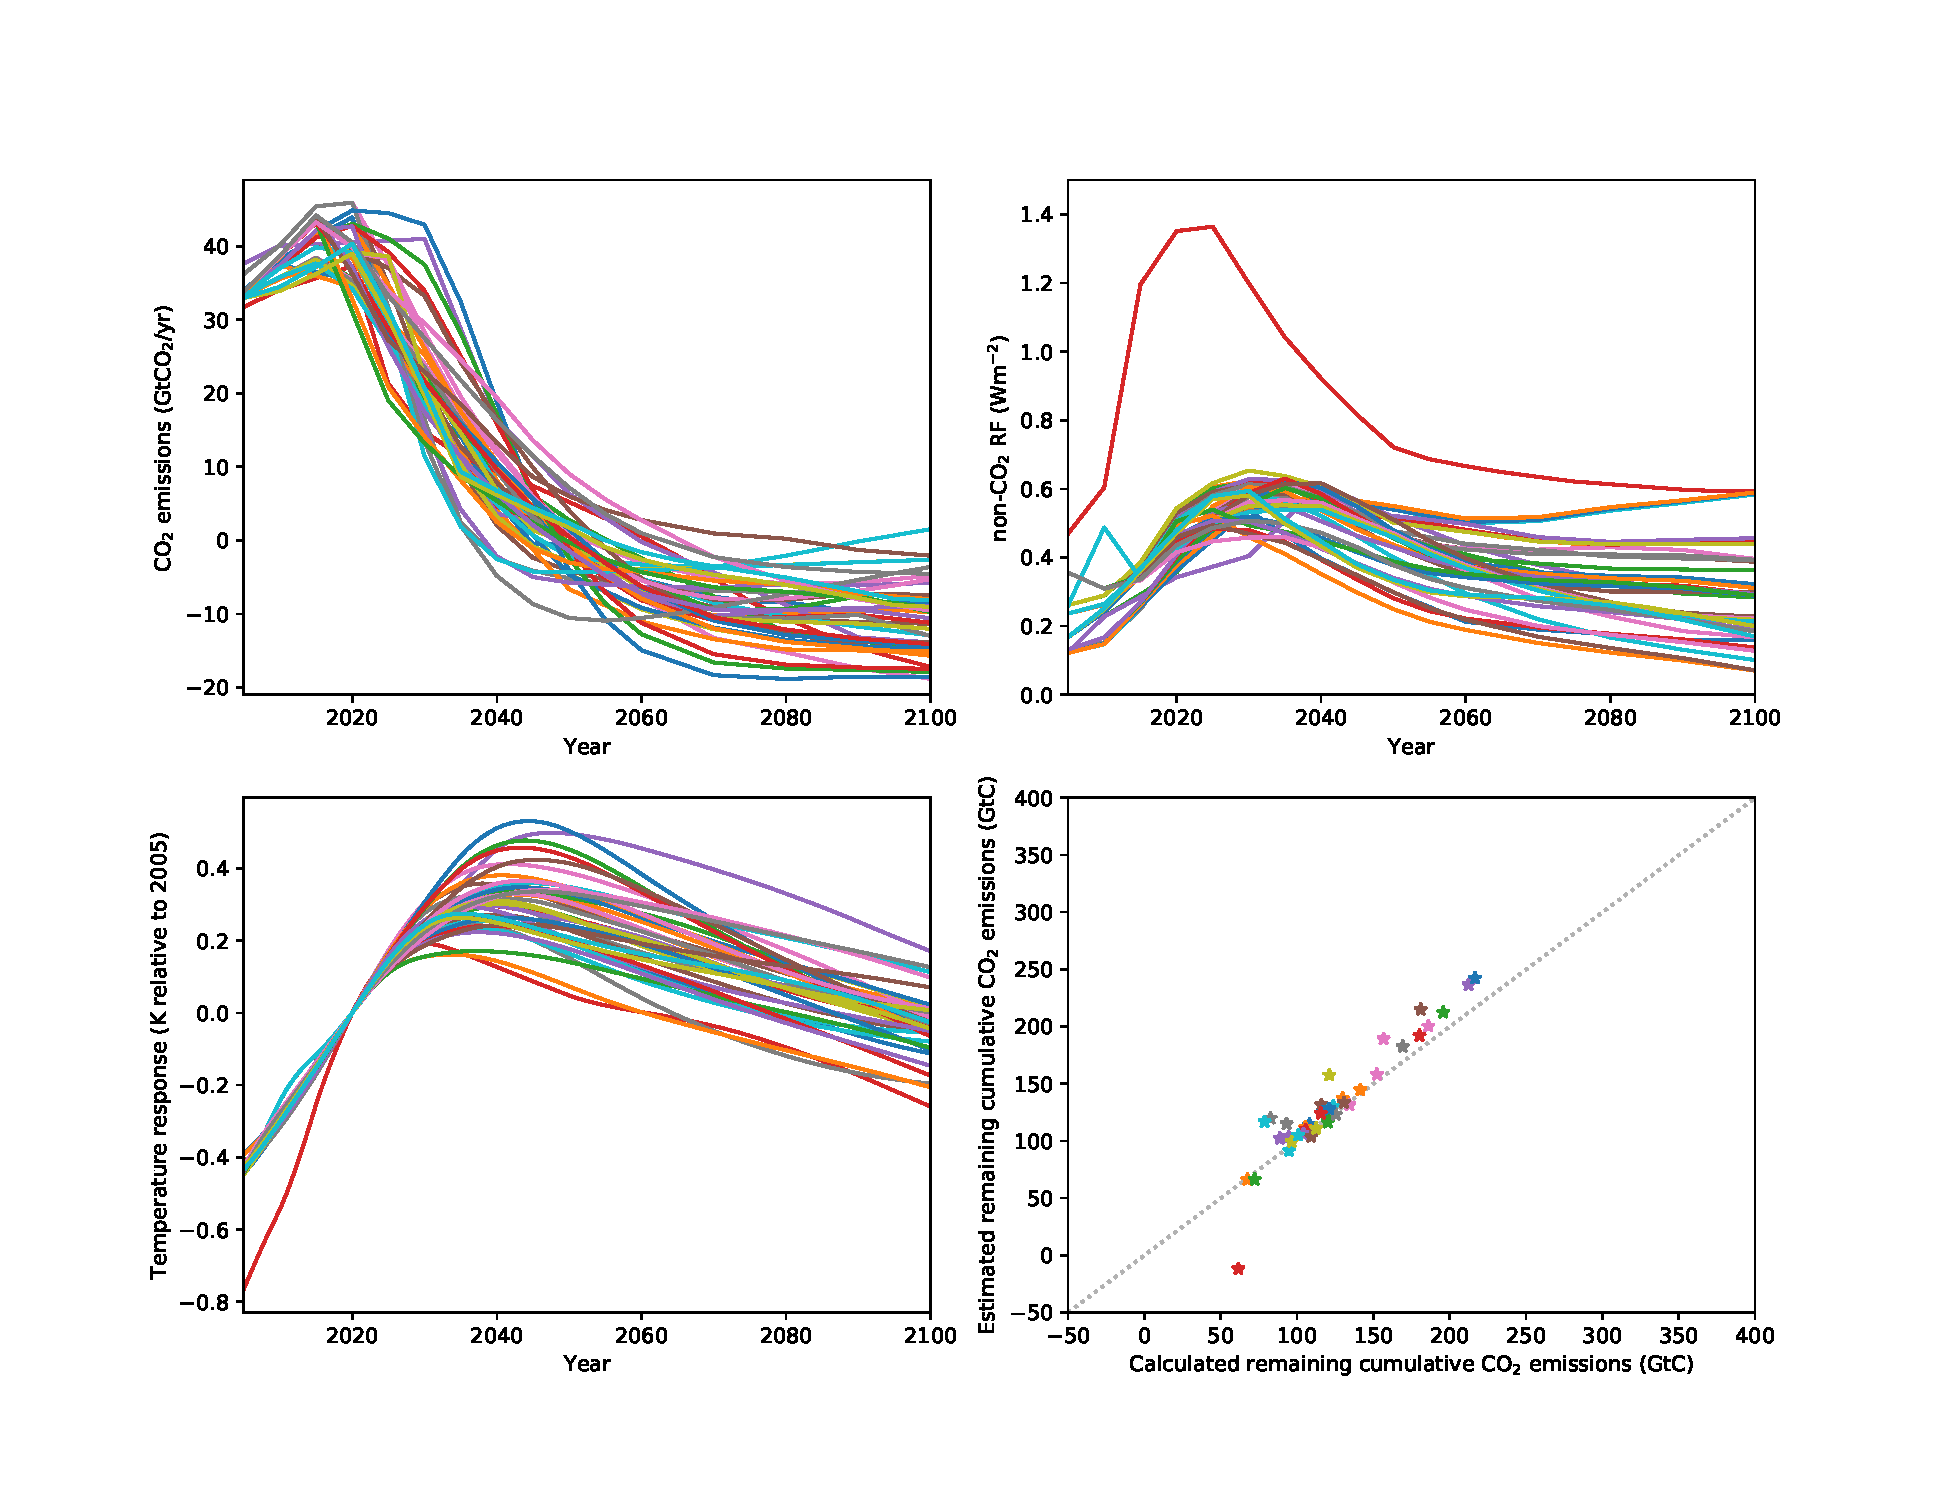
\includegraphics[scale=0.6]{figures/all_scens_tcr175ecs260.pdf}
    \caption{IIASA database 1.5$^{\circ}$C-compatible (no-overshoot/low-overshoot/high-overshoot) scenarios are plotted in panels a (CO$_2$ emissions) and b (non-CO$_2$ radiative forcing). Each scenario is run through the FaIR SCM to find its temperature response (panel c) and time to peak warming. These (with assumptions of the value of TCR, ECS, AGWP$_\text{H}$, d$_2$) are used to estimate the remaining CO$_2$ emissions to peak warming. In Panel d, these estimates are compared with the calculated remaining emissions to peak warming from each scenario in panel a.}
    \label{proofOfConcept}
\end{centering}
\end{figure}

\newpage

\section{The uncertainty in climate response parameters}

The remaining carbon budget to peak warming in these scenarios can be well approximated by equation \ref{cum_carbon_eq} (see figure \ref{proofOfConcept}d). We now explore the effect of varying the climate parameters and other key variables. Figure \ref{paramChoiceEffect}a shows the average estimated against calculated carbon budget for the full range of scenarios in figure \ref{proofOfConcept} for a number of possible TCR (stars) and ECS (circles) choices. Colour groups (reds/greens/blues) show the effect of varying the time period over which the average non-CO$_2$ forcing (F$_0$ and F$_1$) is taken. The three groups of points show the calculation for start years in 2020, 2025 and 2030. 

Figure \ref{paramChoiceEffect}b shows the scenarios average remaining warming to peak warming against calculated carbon budget to peak warming, for the range of TCR and ECS parameters. The dashed lines show the TCRE range. Warming is higher than expected CO$_2$-only warming because of the contribution from non-CO$_2$ forcing. Here it is clear the impact of TCR/ECS choice. The TCR/ECS parameter values don't significantly impact the estimated remaining budget (figure \ref{paramChoiceEffect}a), and as expected up to peak warming date the ECS parameter choice has relatively little impact on warming level for such ambitious mitigation scenarios. TCR is the most significant choice here for determining the remaining warming for a given quantity of carbon emissions (see figure \ref{paramChoiceEffect}b).

\begin{figure}[h]
\begin{centering}
    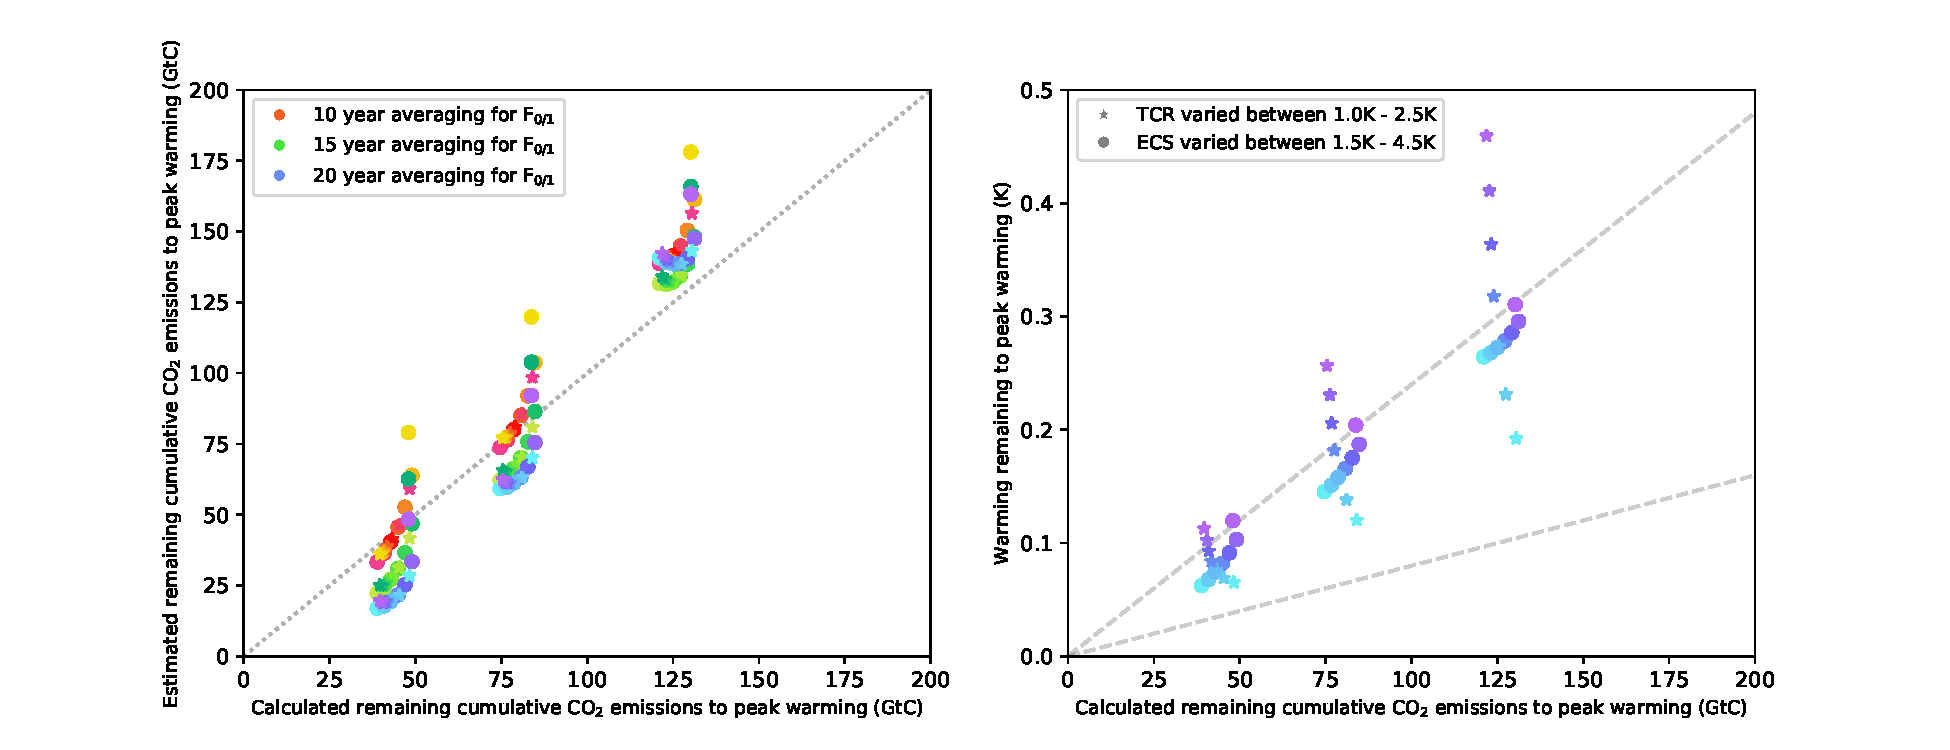
\includegraphics[scale=0.6]{figures/test_all_multiple_startyrs.pdf}
    \caption{Panel a -- IIASA database 1.5$^{\circ}$C-compatible scenarios (plotted in figure \ref{proofOfConcept}a,b) are run through FaIR with set of climate parameters to find the temperature response and estimated remaining CO$_2$ emissions to peak warming. Average of all scenarios remaining budgets are plotted for range of TCR and ECS values (circles and stars, where gradient of colour shows range of values). Reds/greens/blues demonstrate effect of changing period over which averaging non-CO$_2$ forcing is completed: 10, 15 or 20 years. Groups show effect of changing start year for calculation: 2020, 2025 or 2030. Panel b -- FaIR derived remaining warming to peak warming plotted against calculated remaining carbon budget to peak warming for a range of TCR (stars) and ECS (circles) values.}
    \label{paramChoiceEffect}
\end{centering}
\end{figure}

\newpage

\section{Other figures}

\begin{figure}[h]
\begin{centering}
    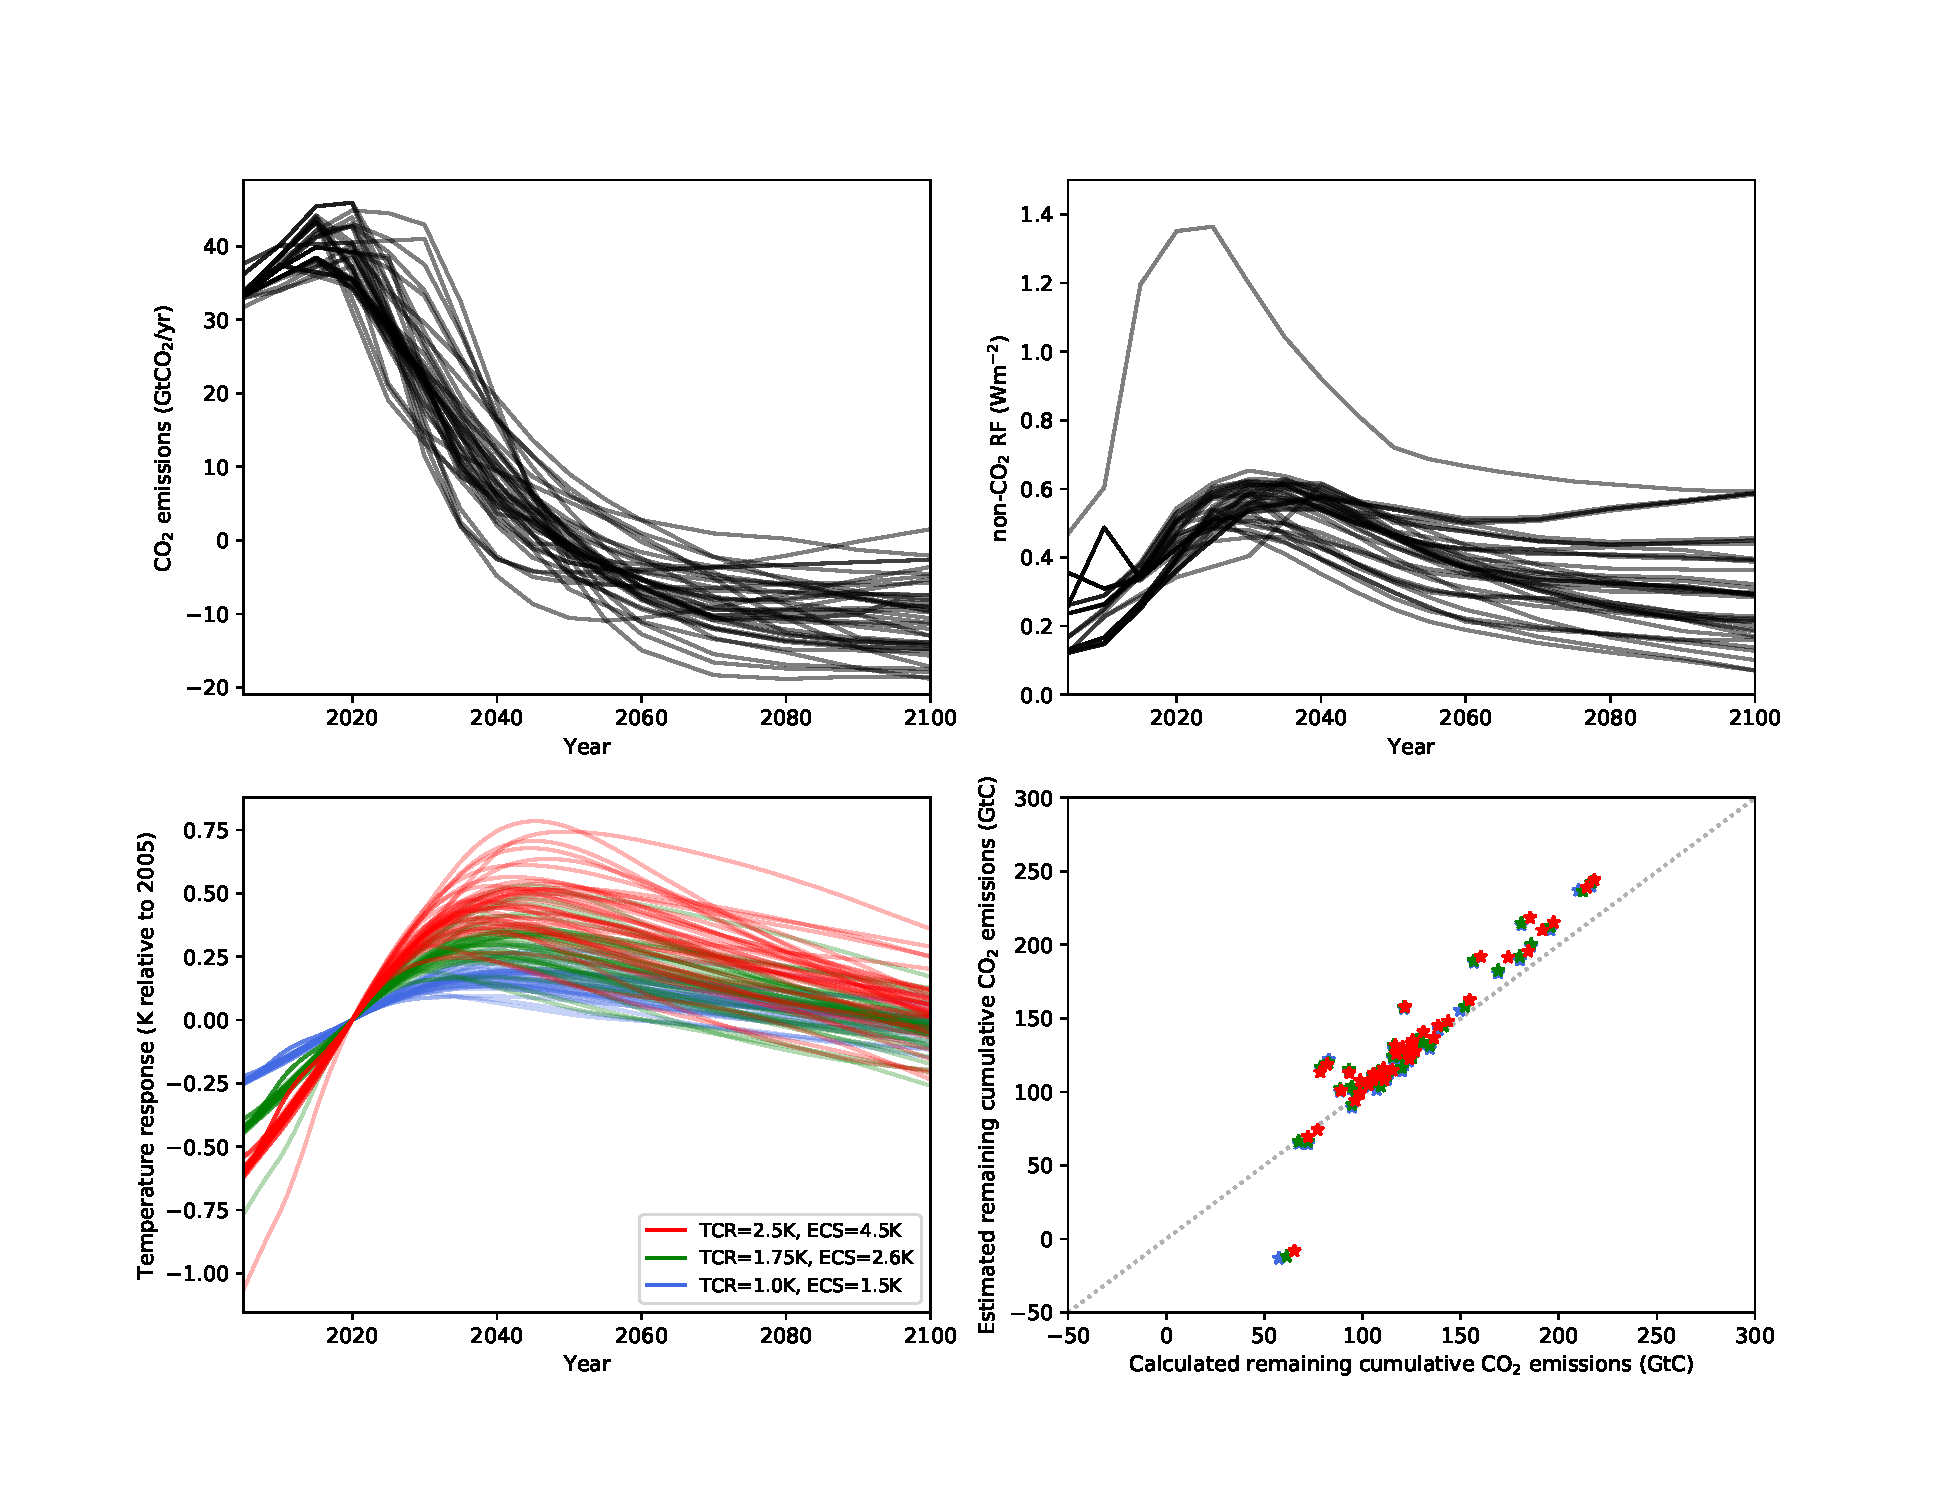
\includegraphics[scale=0.6]{figures/all_scens_tcr_ecs_range.pdf}
    \caption{}
    \label{}
\end{centering}
\end{figure}

\end{document}
